\documentclass[border=3pt]{standalone}
\usepackage{xcolor}
\usepackage{tikz}
\usetikzlibrary{spy}

\begin{document}
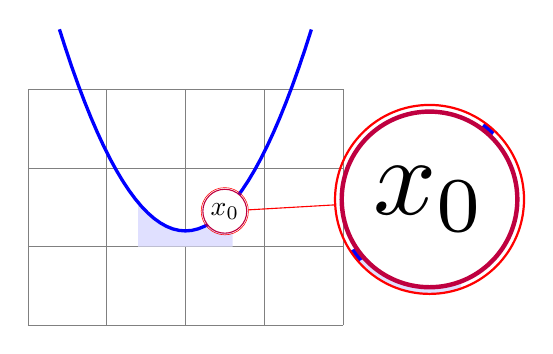
\begin{tikzpicture}[spy using outlines={circle,magnification=4,size=2.4cm,connect spies}]
  \draw[help lines] (-2,-1) grid (2,2);
  \fill[blue!12] (-.6,0) -- plot[domain=-.6:.6,samples=31] (\x,{\x*\x+.2}) -- (.6,0) -- cycle;
  \draw[blue,very thick] plot[domain=-1.6:1.6,samples=41] (\x,{\x*\x+.2});
  \node[draw=purple,fill=white,circle,inner sep=1.5pt] at (.5,.45) {$x_0$};
  \spy[red] on (.5,.45) in node at (3.1,.6);
\end{tikzpicture}
\end{document}
